%=== Préambule ===========================================================

\documentclass{beamer}
\usepackage{pdfpages}
\usepackage[english]{babel}
\usepackage{xspace}
\usepackage{pifont}
\usepackage{hyperref}
\usepackage{listings}
\usepackage{csquotes}
\usepackage{graphicx}
\usepackage{animate,media9} %,movie15}
\usepackage{wrapfig}
\usepackage{pdfpages}
\usepackage{tikz}
\usepackage{natbib}
\uselanguage{English}
\usepackage{fontawesome5}
\languagepath{English}
\setcounter{tocdepth}{1}
\usepackage{setspace}
\usepackage{amsmath}
\def\glasses{{\sffamily 
\leavevmode\rlap{%
\rotatebox[origin=tr]{125}{J}\kern1ex%  
\rotatebox[origin=tr]{125}{J}}% 
\rotatebox[origin=c]{-90}{D}%   
\rotatebox[origin=c]{-90}{D}}%
\def\ialy{\sffamily 
\resizebox{1ex}{1.5ex}{\reflectbox{\rotatebox[origin=]{75}{J}}}\kern-1pt%
\rlap{\tiny$\ ^\bullet\kern2.5pt^\bullet$ }%
\rotatebox[origin=c]{-90}{D}%   
\rotatebox[origin=c]{-90}{D}\kern-1pt%  
\resizebox{1ex}{1.5ex}{\rotatebox[origin=]{75}{J}}}}


\lstset{
  numbers=left,
  basicstyle=\tiny\ttfamily,      
  breaklines=true, 
  showtabs=false,
  showstringspaces=false,
}  

%=== Configuration de Beamer et du thème metropolis ======================
\usepackage{bbding}
\usetheme[background=light]{metropolis}
\usepackage[clock]{ifsym}

\definecolor{mLightBrown}{HTML}{000000}
\definecolor{black}{HTML}{000000}
\setbeamercolor{structure}{fg=black,bg=mLightBrown}
\setbeamercolor{palette primary}{%
	use=normal text,
	fg=normal text.bg,
	bg=mLightBrown
}
%\setsansfont[BoldFont={Linux Libertine G Bold},Numbers={OldStyle}]{Linux Libertine G}

\metroset{block=fill}

%=== Page de titre =======================================================

%path to logo and biblio -> to be adapted to your local directories 
\newcommand\dirlogo{../../logos/}
\newcommand\dirbiblio{../../biblio}



\title{{\normalsize \vskip 1cm Seminario: Filtro R\'apido de Coincidencias \\ \hskip 2cm ``Fast Matched Filter"}}
\subtitle{\small Posibles aplicaciónes a microsismicidad}
\author{Hugo S. \\ {\tiny Institut de Recherche pour le Développement IRD - ISTerre} \\ 
\\
Gracias a mis colegas: \\
P. Poli, L. Cabrera, D. Essing, A. Socquet, H. Tavera, E. Beauc\'e \\
\\
\textit{Seminario en el IGP, LabEx OSUG Project EFASAP}
}

\date[2022]{\today}

\subject{Group Meeting}

\titlegraphic{\centering \vspace{-18pt}
\includegraphics[height=1.2cm]{../../../logos/logo_seminar_2022.pdf} \par} %\qquad  
\includegraphics[height=1.4cm]{../../logos/anr_eqtime.png} \par }


\addtobeamertemplate{frametitle}{}{%
\begin{tikzpicture}[remember picture,overlay]
  \node[anchor=north east,yshift=0.0ex] at (current page.north east) {
\includegraphics[height=4ex]{../../../logos/ISTerre_neg.pdf}};
  %\node[anchor=north east,yshift=0.5ex] at (current page.north east) {\includegraphics[height=3.3ex]{\dirlogo/seiscope_color_light_background}};
\end{tikzpicture}}



%=== Document ============================================================

\begin{document}

% --- Préambule ---------------------------------------------------------------

\begin{frame}
    \titlepage
\end{frame}

\section{Introducci\'on}

\begin{frame}
 {Similitud, correlaci\'on}

 \begin{minipage}{0.45\linewidth}
 \centering Manzanas con manzanas \\
            y peras con peras \\
            \vskip 0.3cm
 
\includegraphics[width=0.6\linewidth]{images/apples.png}
 \end{minipage}
 \begin{minipage}{0.4\linewidth}
    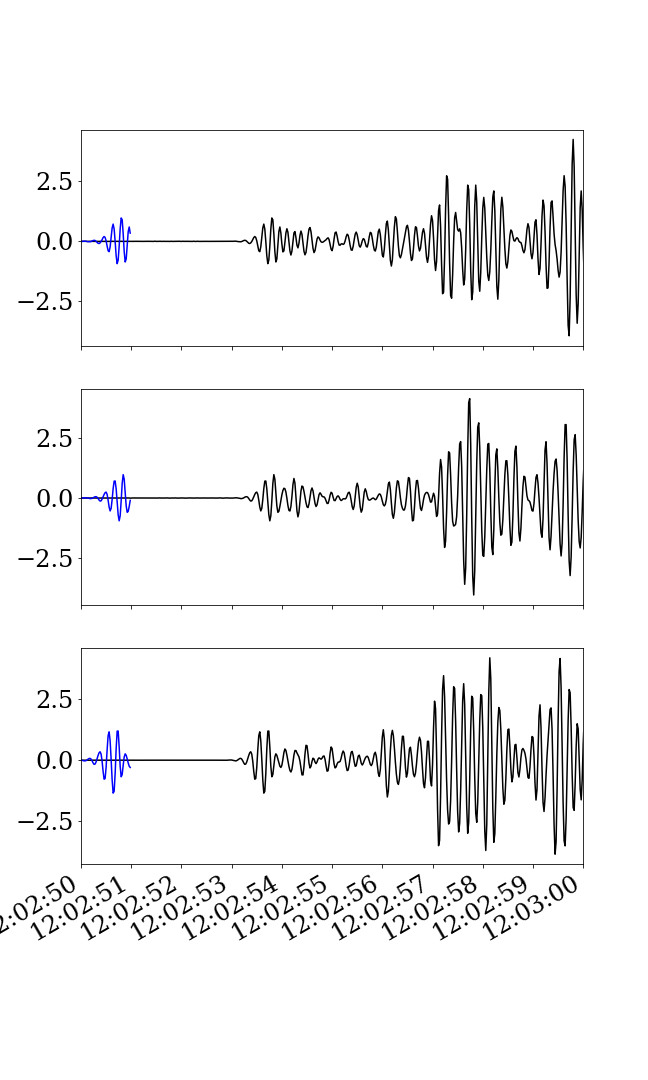
\includegraphics[width=1.2\linewidth]{images/fig_0.png}
 \end{minipage}
 
\end{frame}


\begin{frame}
 {Similitud, correlaci\'on}

 \begin{minipage}{0.45\linewidth}
 \centering Manzanas con manzanas \\
            y peras con peras \\
            \vskip 0.3cm
 
\includegraphics[width=0.6\linewidth]{images/apples.png}
 \end{minipage}
 \begin{minipage}{0.4\linewidth}
    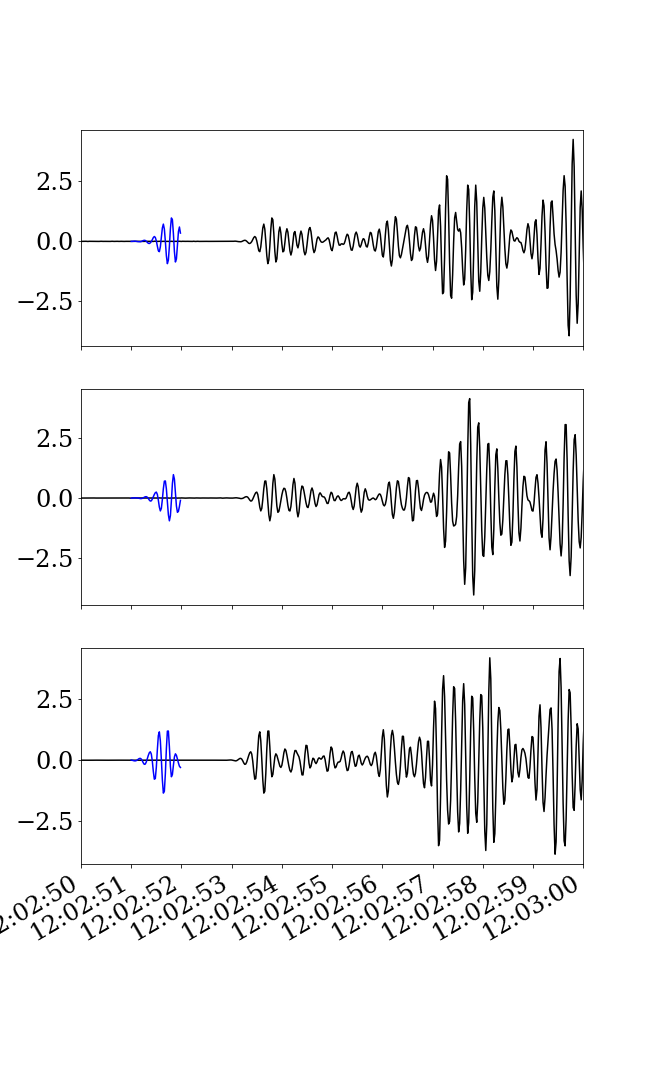
\includegraphics[width=1.2\linewidth]{images/fig_1.png}
 \end{minipage}
 
\end{frame}


\begin{frame}
 {Similitud, correlaci\'on}

 \begin{minipage}{0.45\linewidth}
 \centering Manzanas con manzanas \\
            y peras con peras \\
            \vskip 0.3cm
 
\includegraphics[width=0.6\linewidth]{images/apples.png}
 \end{minipage}
 \begin{minipage}{0.4\linewidth}
    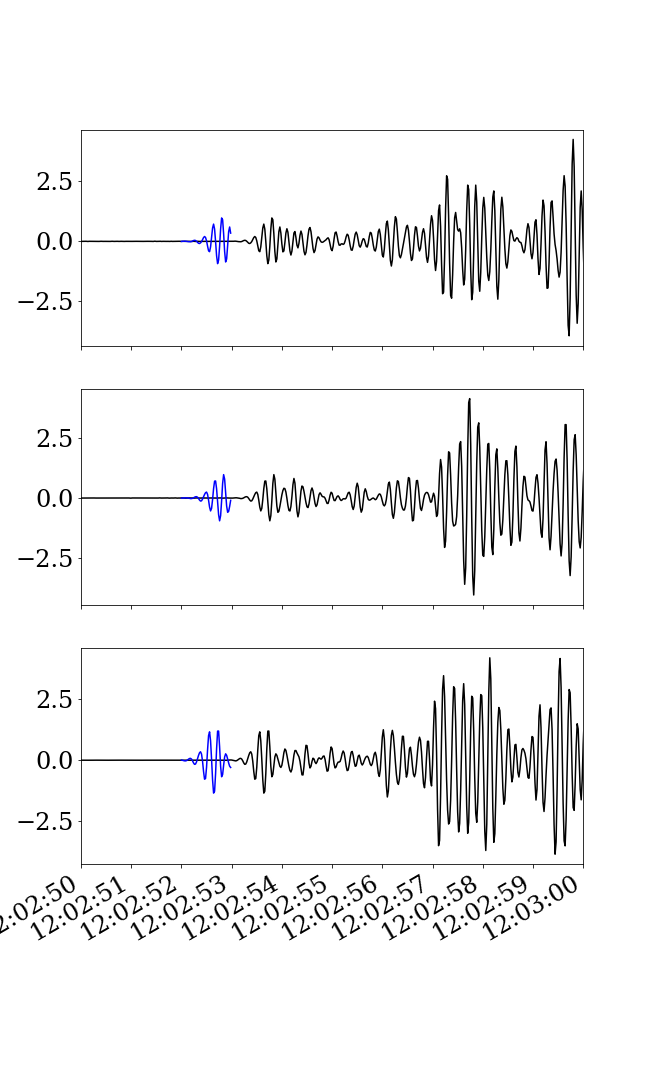
\includegraphics[width=1.2\linewidth]{images/fig_2.png}
 \end{minipage}
 
\end{frame}


\begin{frame}
 {Similitud, correlaci\'on}

 \begin{minipage}{0.45\linewidth}
 \centering Manzanas con manzanas \\
            y peras con peras \\
            \vskip 0.3cm
 
\includegraphics[width=0.6\linewidth]{images/apples.png}
 \end{minipage}
 \begin{minipage}{0.4\linewidth}
    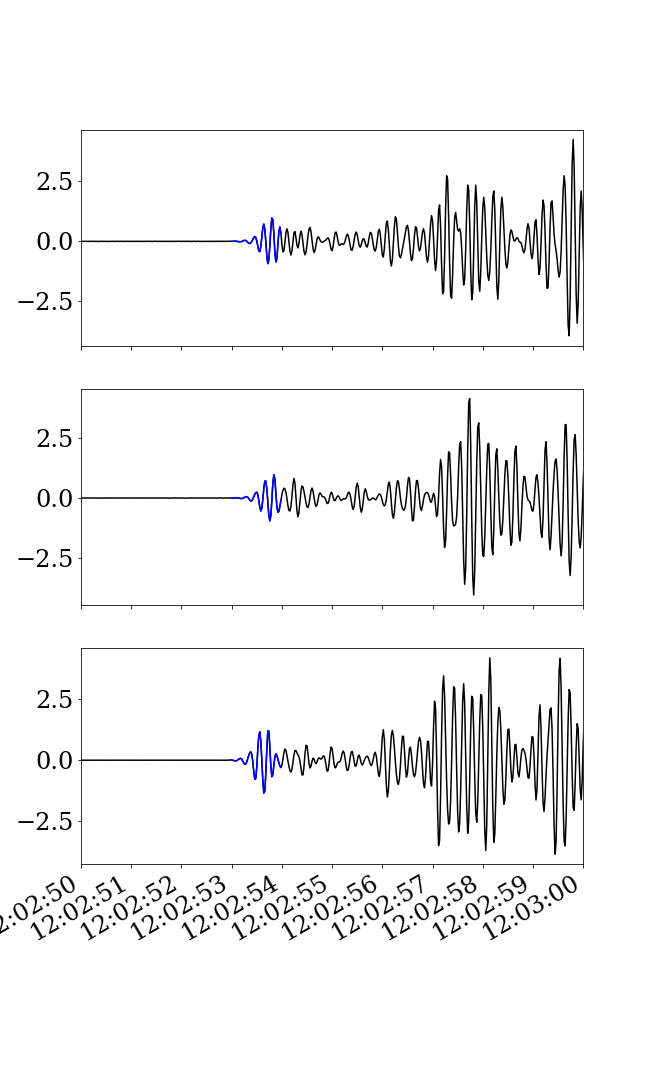
\includegraphics[width=1.2\linewidth]{images/fig_3.png}
 \end{minipage}
 
\end{frame}


\begin{frame}
 {Similitud, correlaci\'on}

 \begin{minipage}{0.45\linewidth}
 \centering Manzanas con manzanas \\
            y peras con peras \\
            \vskip 0.3cm
 
\includegraphics[width=0.6\linewidth]{images/apples.png}
 \end{minipage}
 \begin{minipage}{0.4\linewidth}
    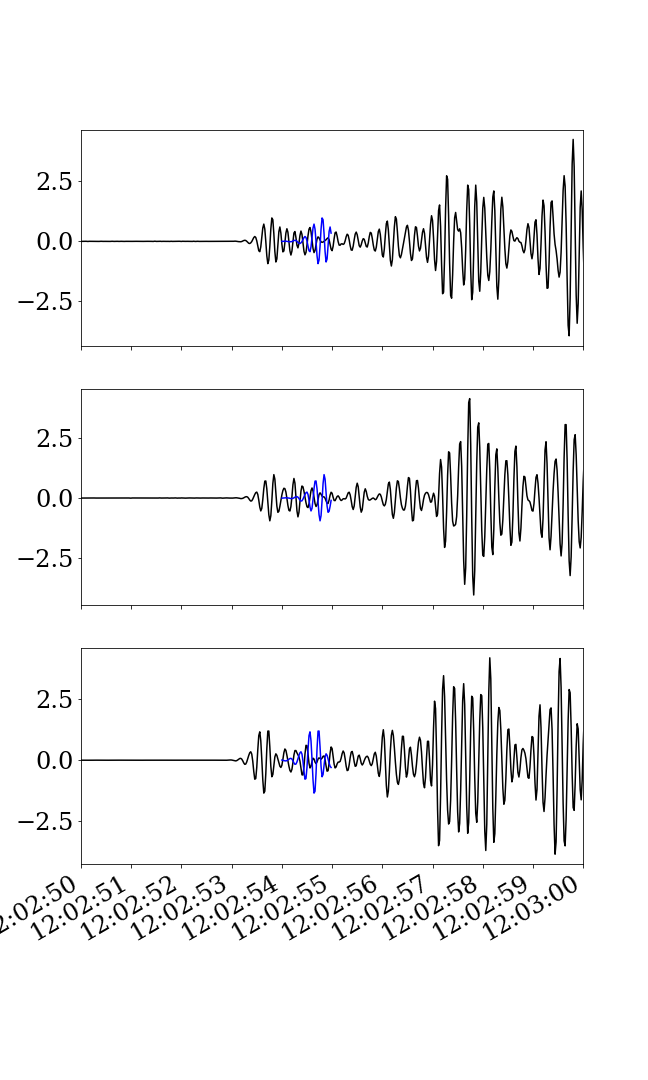
\includegraphics[width=1.2\linewidth]{images/fig_4.png}
 \end{minipage}
 
\end{frame}


\begin{frame}
 {Similitud, correlaci\'on}

 \begin{minipage}{0.45\linewidth}
 \centering Manzanas con manzanas \\
            y peras con peras \\
            \vskip 0.3cm
 
\includegraphics[width=0.6\linewidth]{images/apples.png}
 \end{minipage}
 \begin{minipage}{0.4\linewidth}
    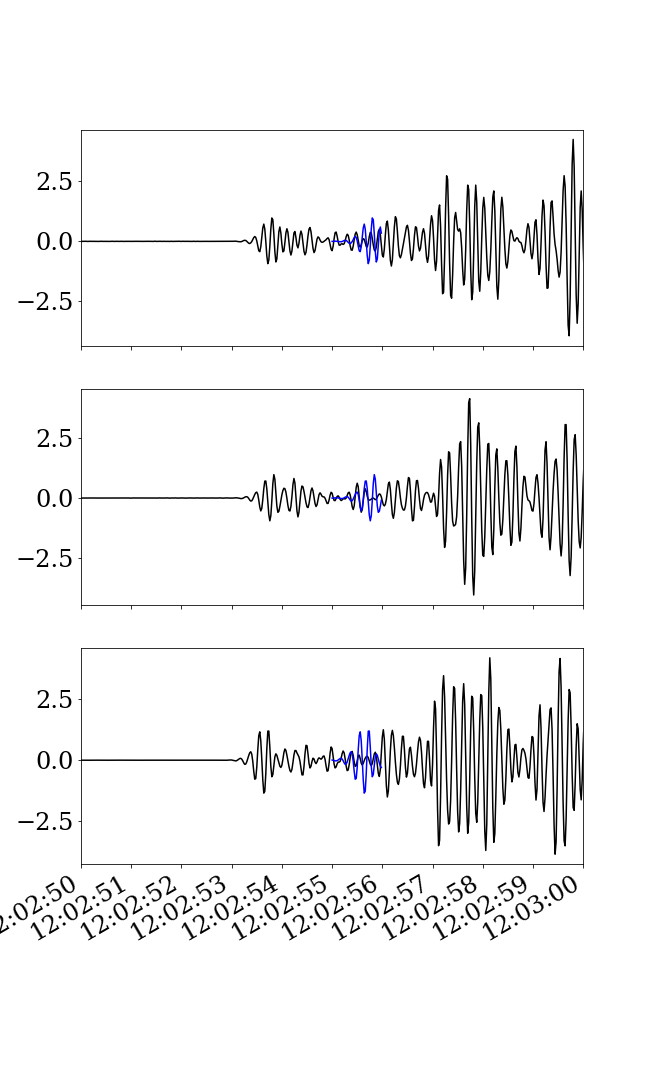
\includegraphics[width=1.2\linewidth]{images/fig_5.png}
 \end{minipage}
 
\end{frame}


\begin{frame}
 {Similitud, correlaci\'on}

 \begin{minipage}{0.45\linewidth}
 \centering Manzanas con manzanas \\
            y peras con peras \\
            \vskip 0.3cm
 
\includegraphics[width=0.6\linewidth]{images/apples.png}
 \end{minipage}
 \begin{minipage}{0.4\linewidth}
    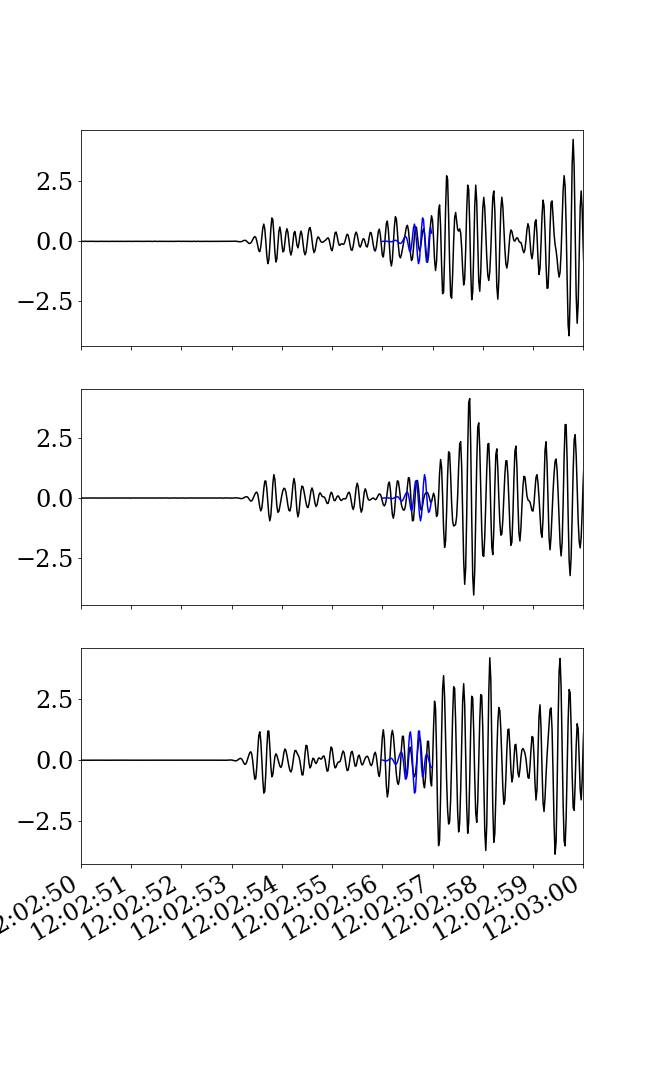
\includegraphics[width=1.2\linewidth]{images/fig_6.png}
 \end{minipage}
 
\end{frame}


\begin{frame}
 {Similitud, correlaci\'on}

 \begin{minipage}{0.45\linewidth}
 \centering Manzanas con manzanas \\
            y peras con peras \\
            \vskip 0.3cm
 
\includegraphics[width=0.6\linewidth]{images/apples.png}
 \end{minipage}
 \begin{minipage}{0.4\linewidth}
    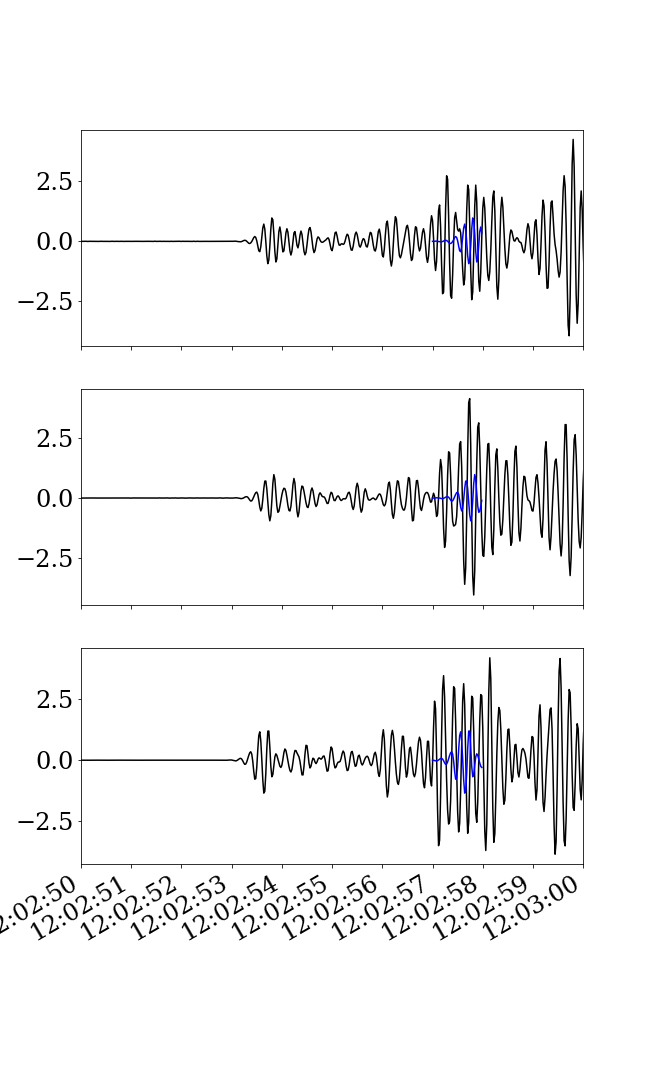
\includegraphics[width=1.2\linewidth]{images/fig_7.png}
 \end{minipage}
 
\end{frame}


\section{Instalaci\'on}




\begin{frame}
{Creaci\'on de ambiente de trabajo ''fmf\_tuto"}

 \centering
 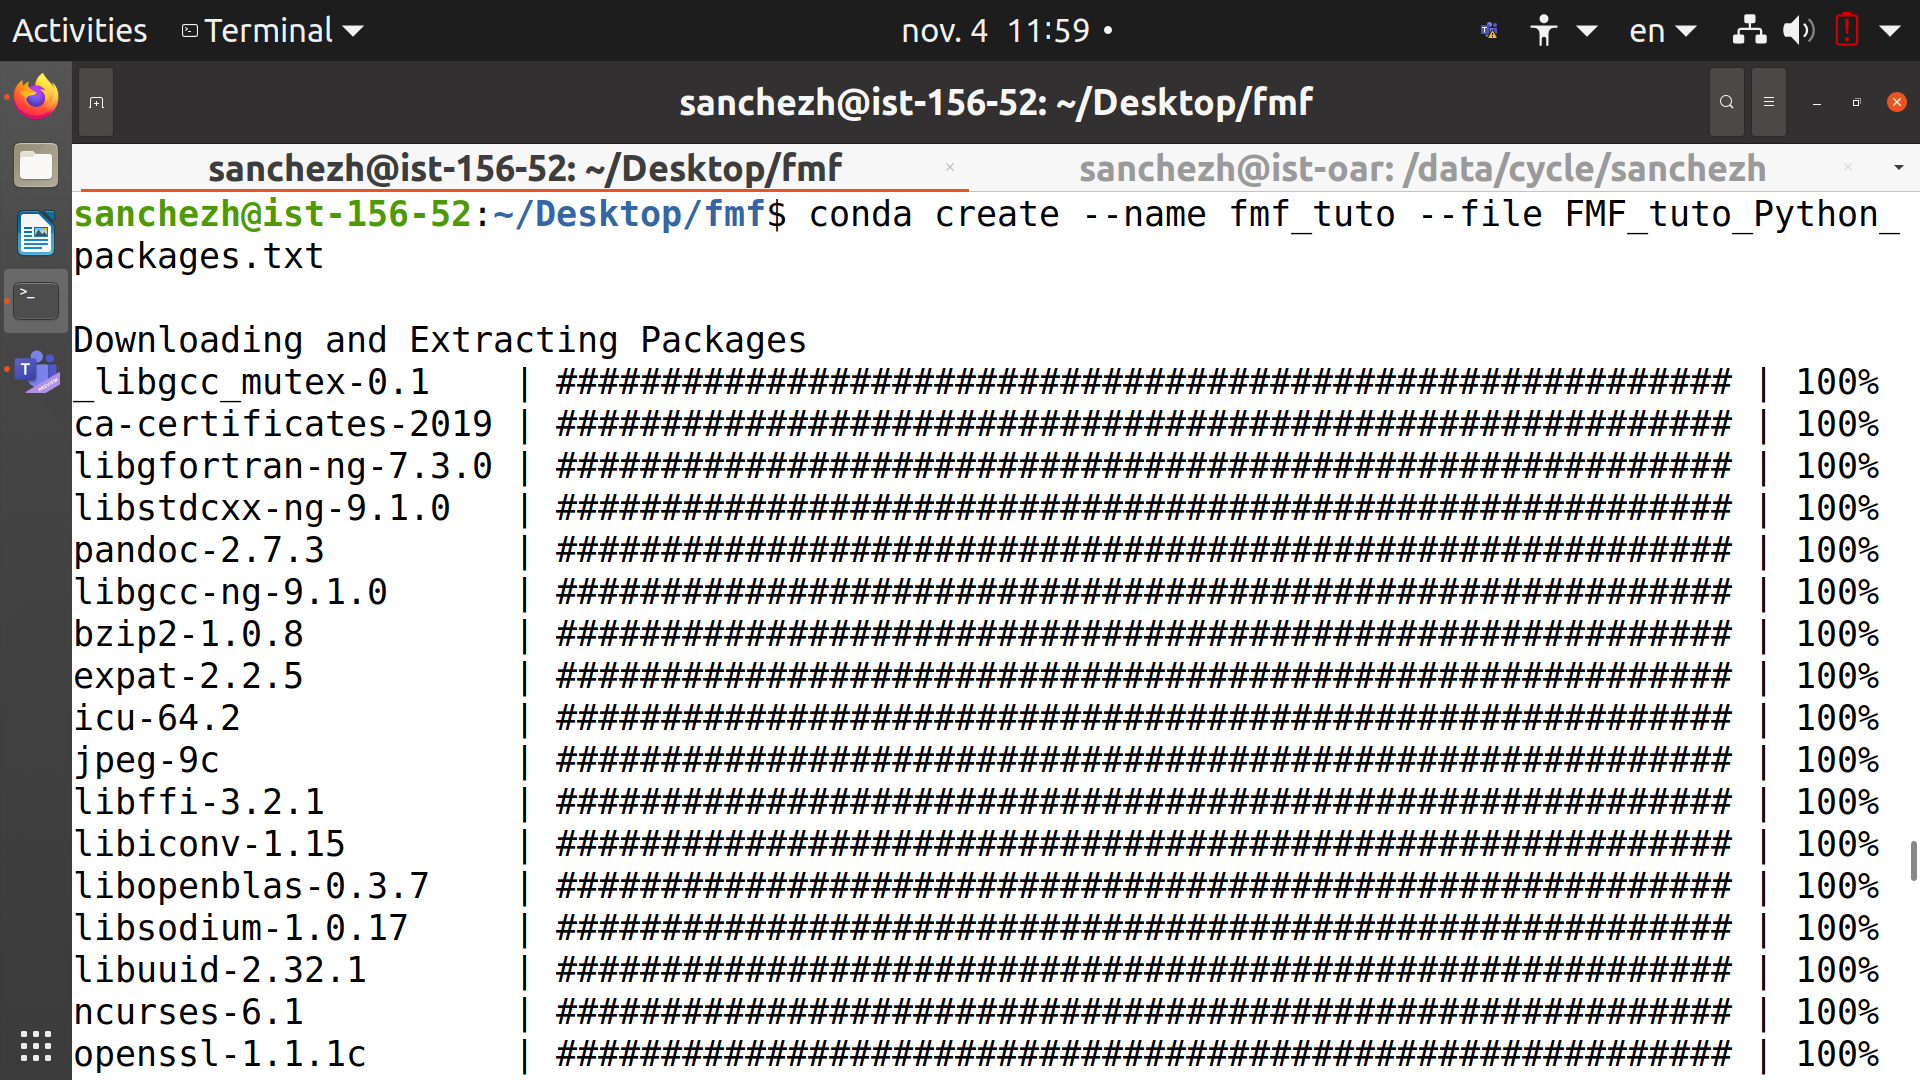
\includegraphics[width=1\linewidth]{images/conda_create_fmf.png}
 
\end{frame}

\begin{frame}
 {Instalaci\'on de ``ObsPy"}
 
 \centering
 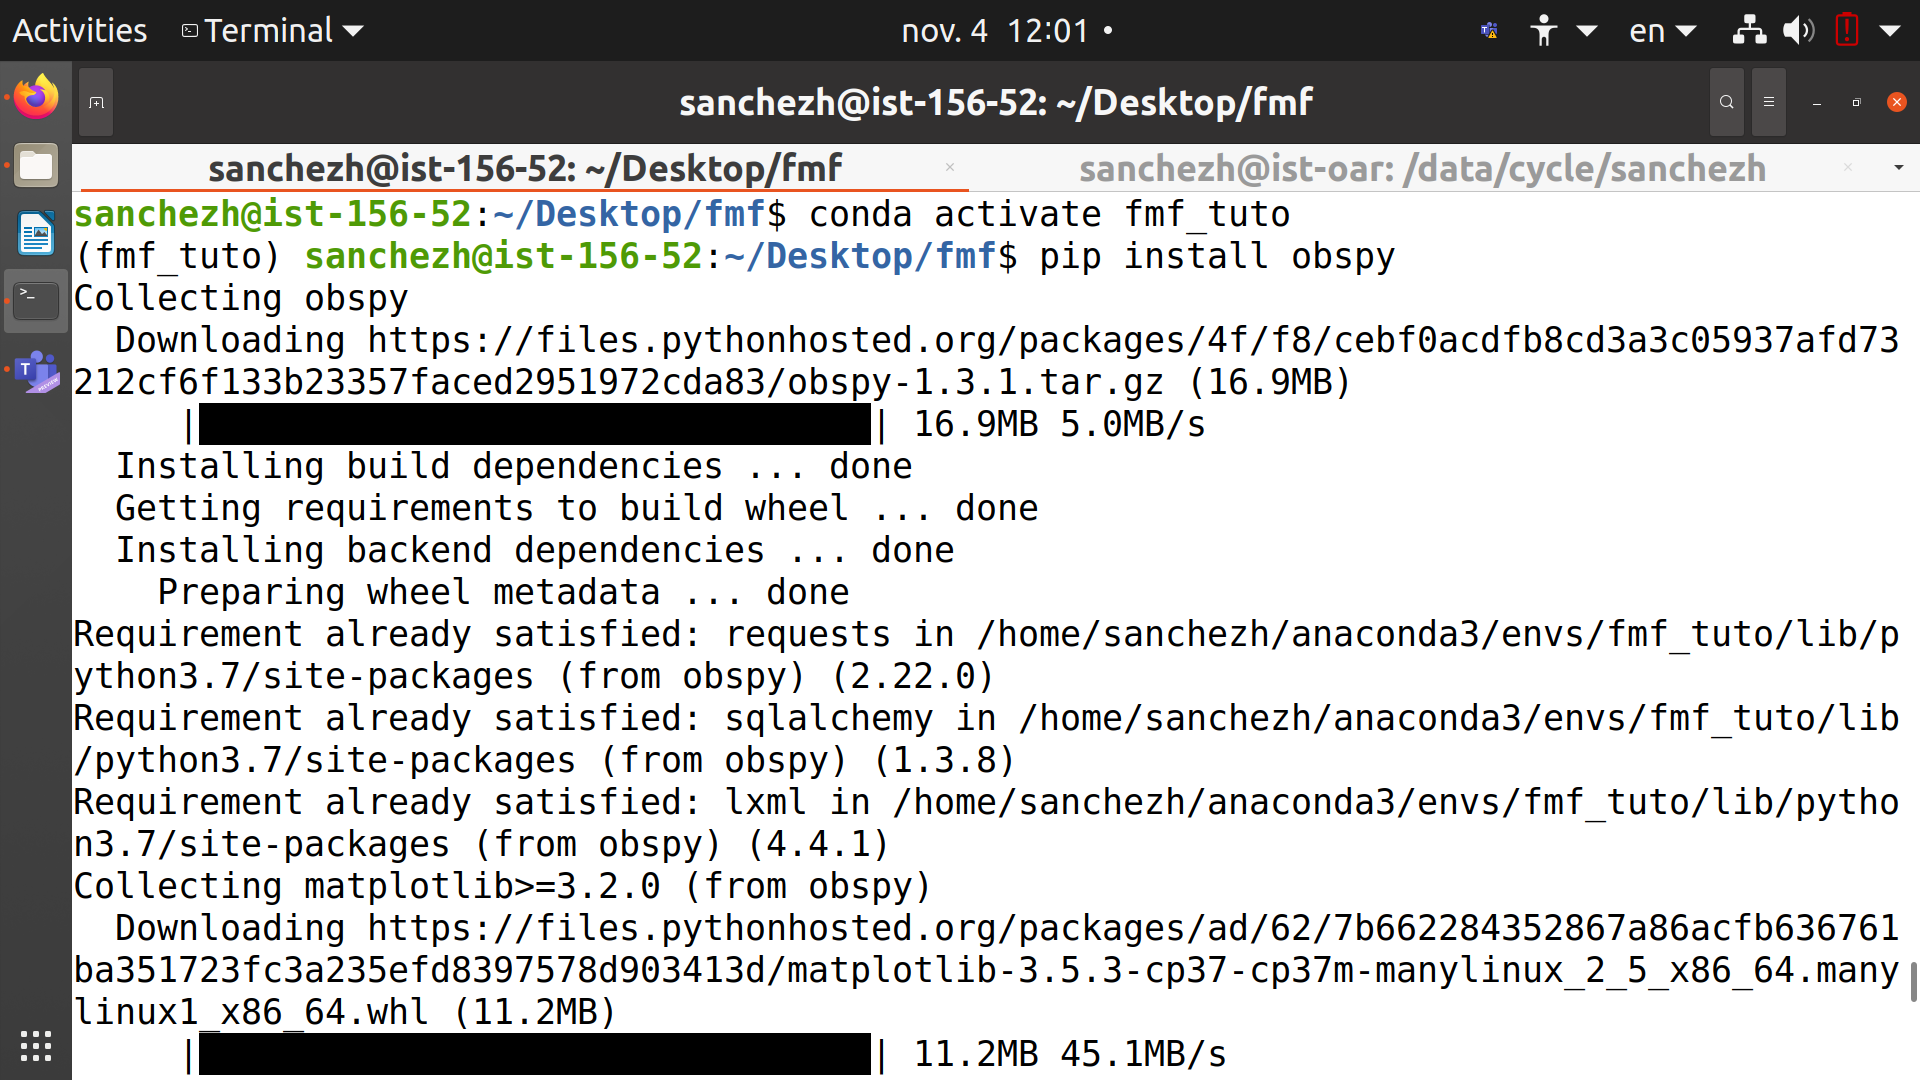
\includegraphics[width=1\linewidth]{images/conda_activate_fmf_install_obspy.png}
 
\end{frame}

\begin{frame}
 {Instalaci\'on de ``ObsPy"}
 
 \centering
 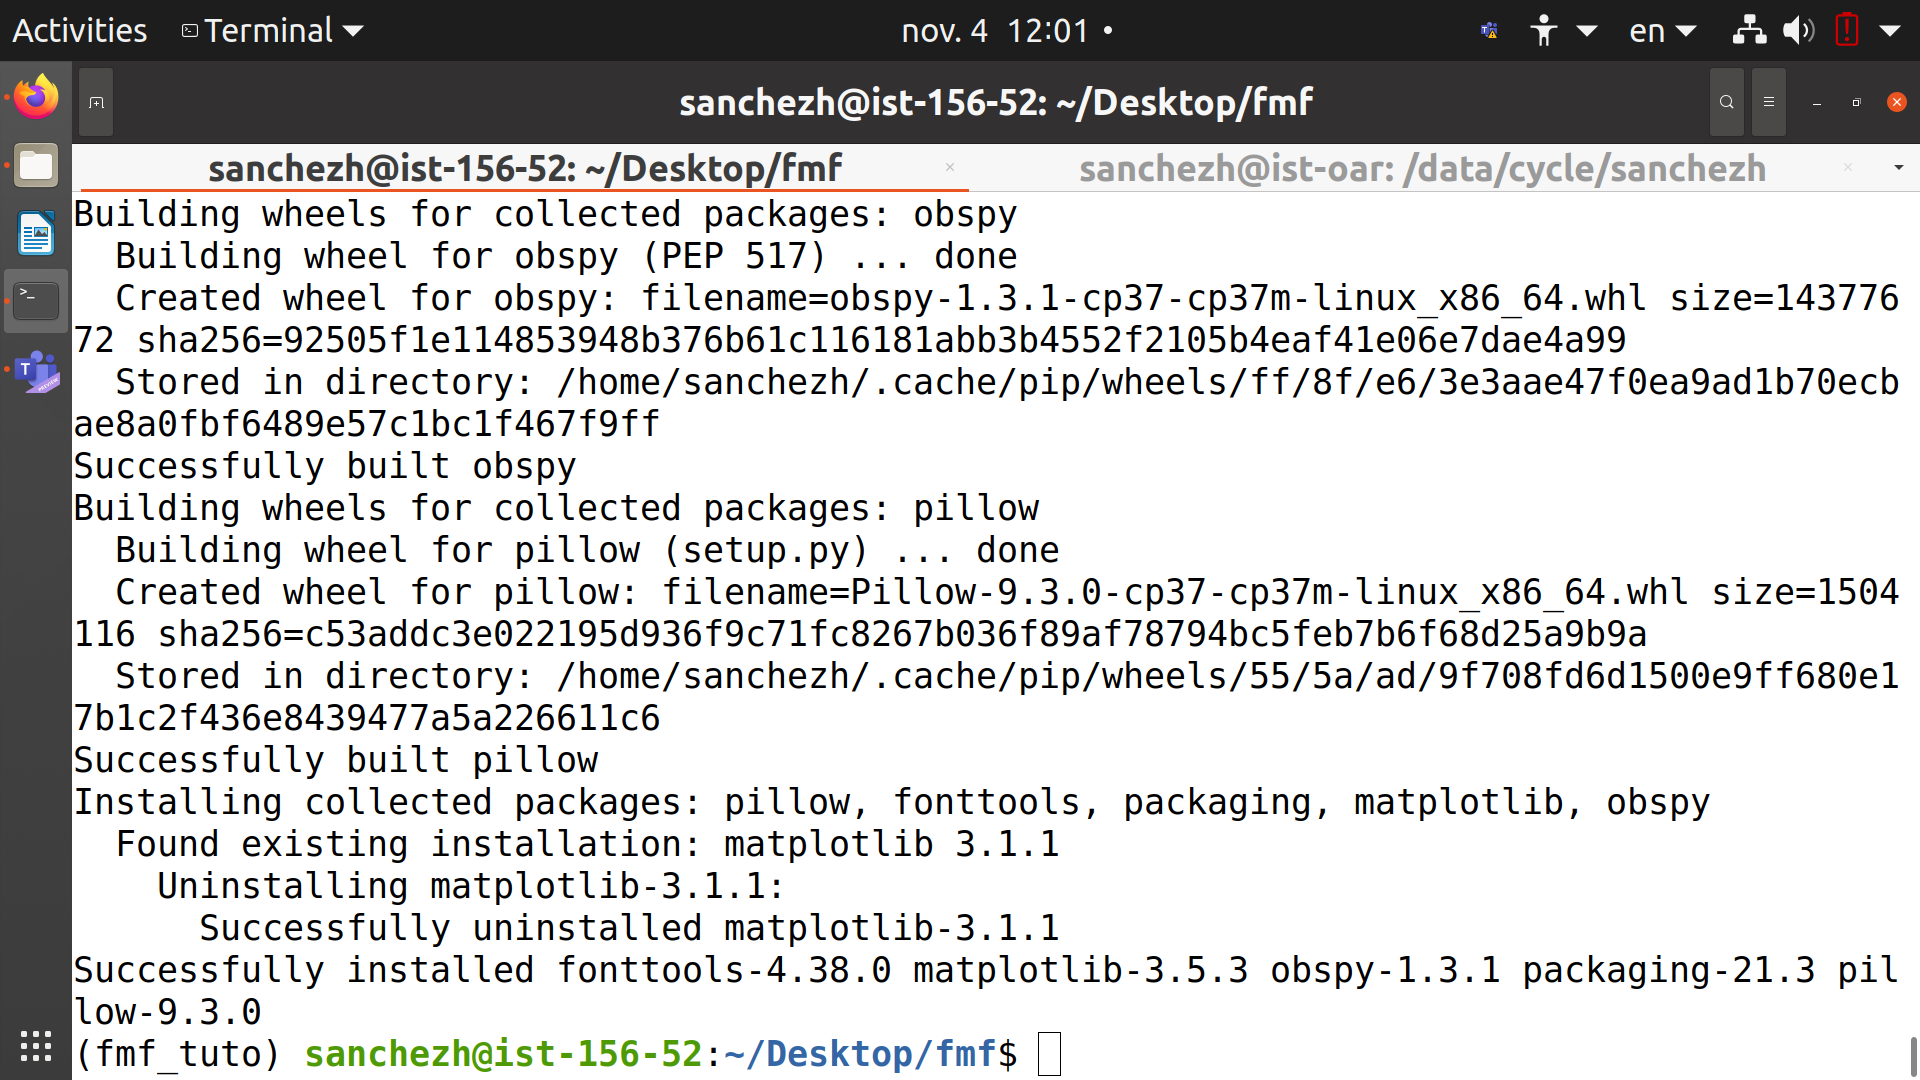
\includegraphics[width=1\linewidth]{images/succes_install_obspy.png}
 
\end{frame}


\begin{frame}
 {Abrir ''jupyter notebook"}

 \centering
 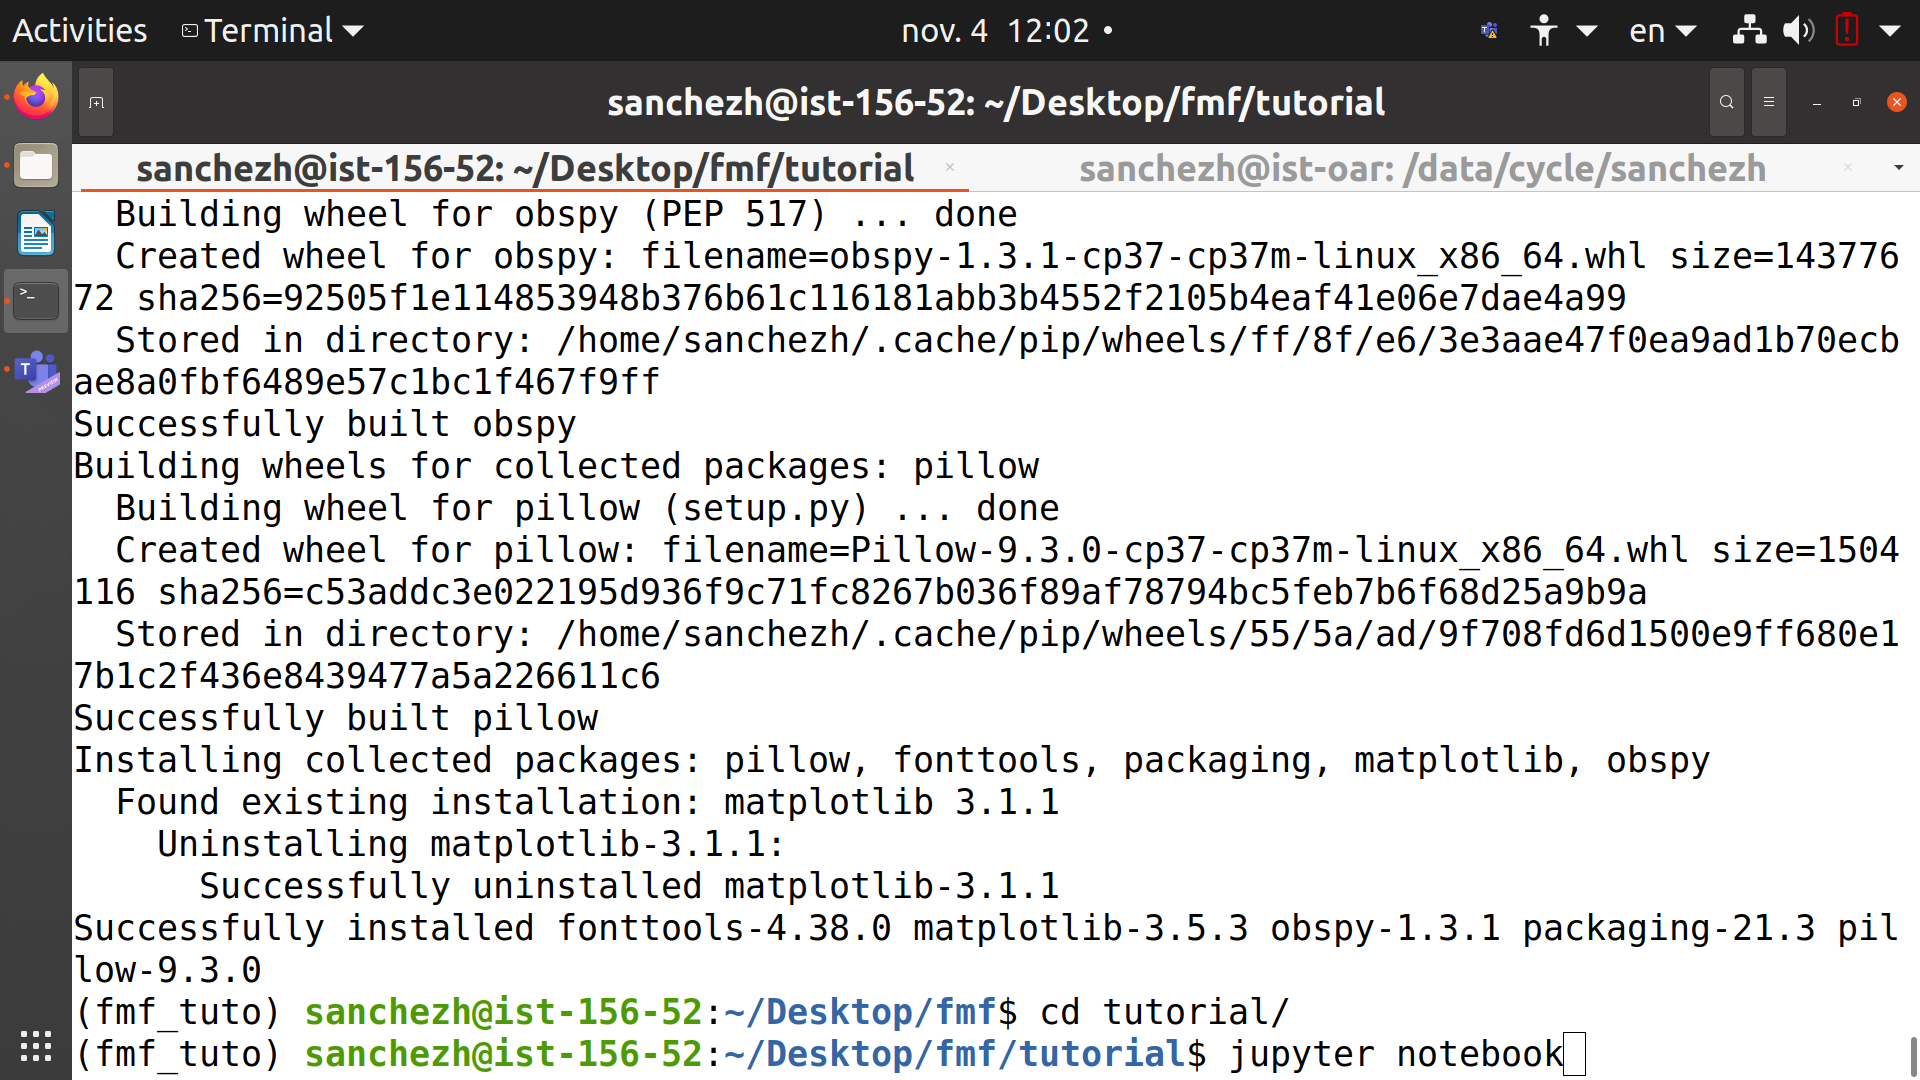
\includegraphics[width=1\linewidth]{images/jupyter_notebook.png}
 
\end{frame}



\section{Ejemplo}

\begin{frame}
 {Secuencia s\'ismica del sismo 2019 Mw4 Balsorano, Italia}

 \begin{minipage}{1\linewidth}
  \centering 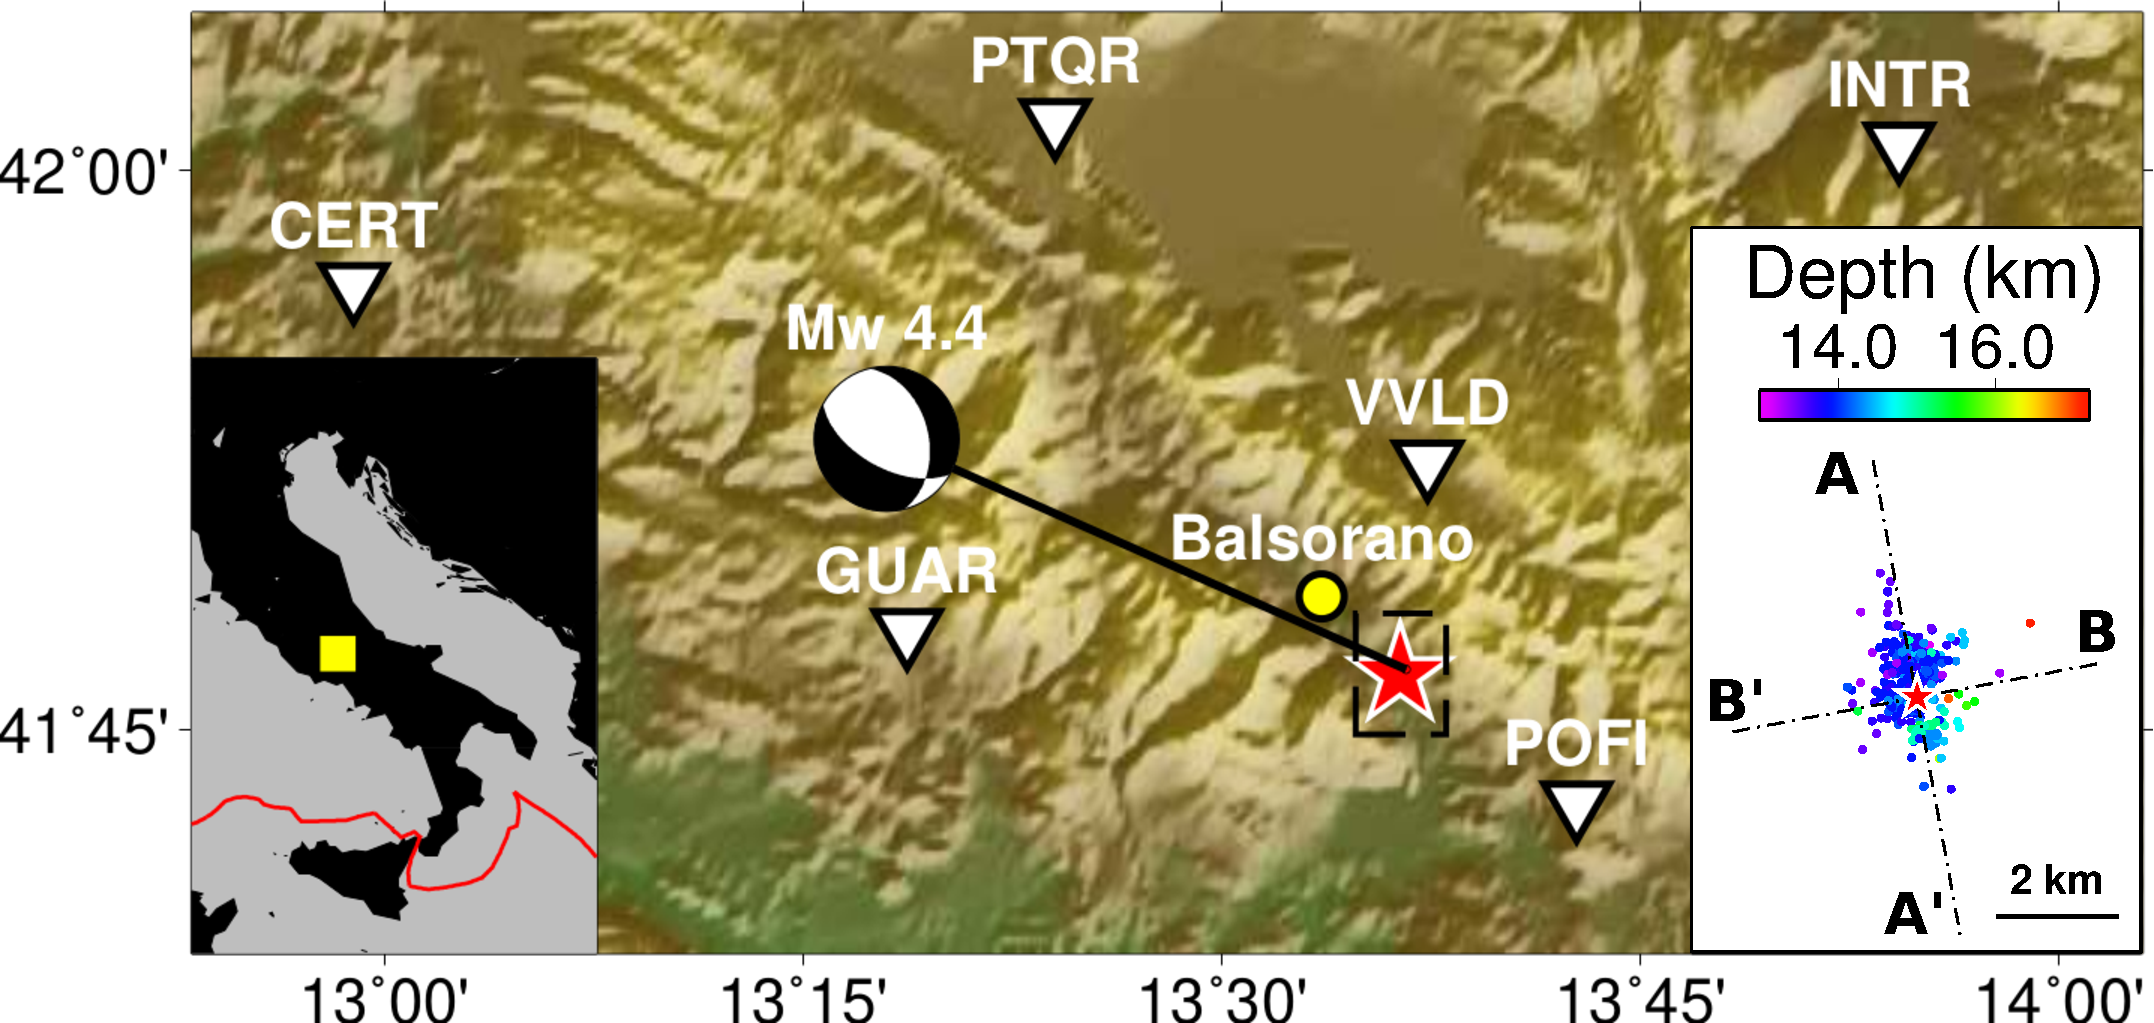
\includegraphics[width=1\linewidth]{images/map_balsorano.pdf}
 \end{minipage} 
 
\end{frame}


\begin{frame}
 {Secuencia s\'ismica del sismo 2019 Mw4 Balsorano, Italia}

 \begin{minipage}{1\linewidth}
  \centering 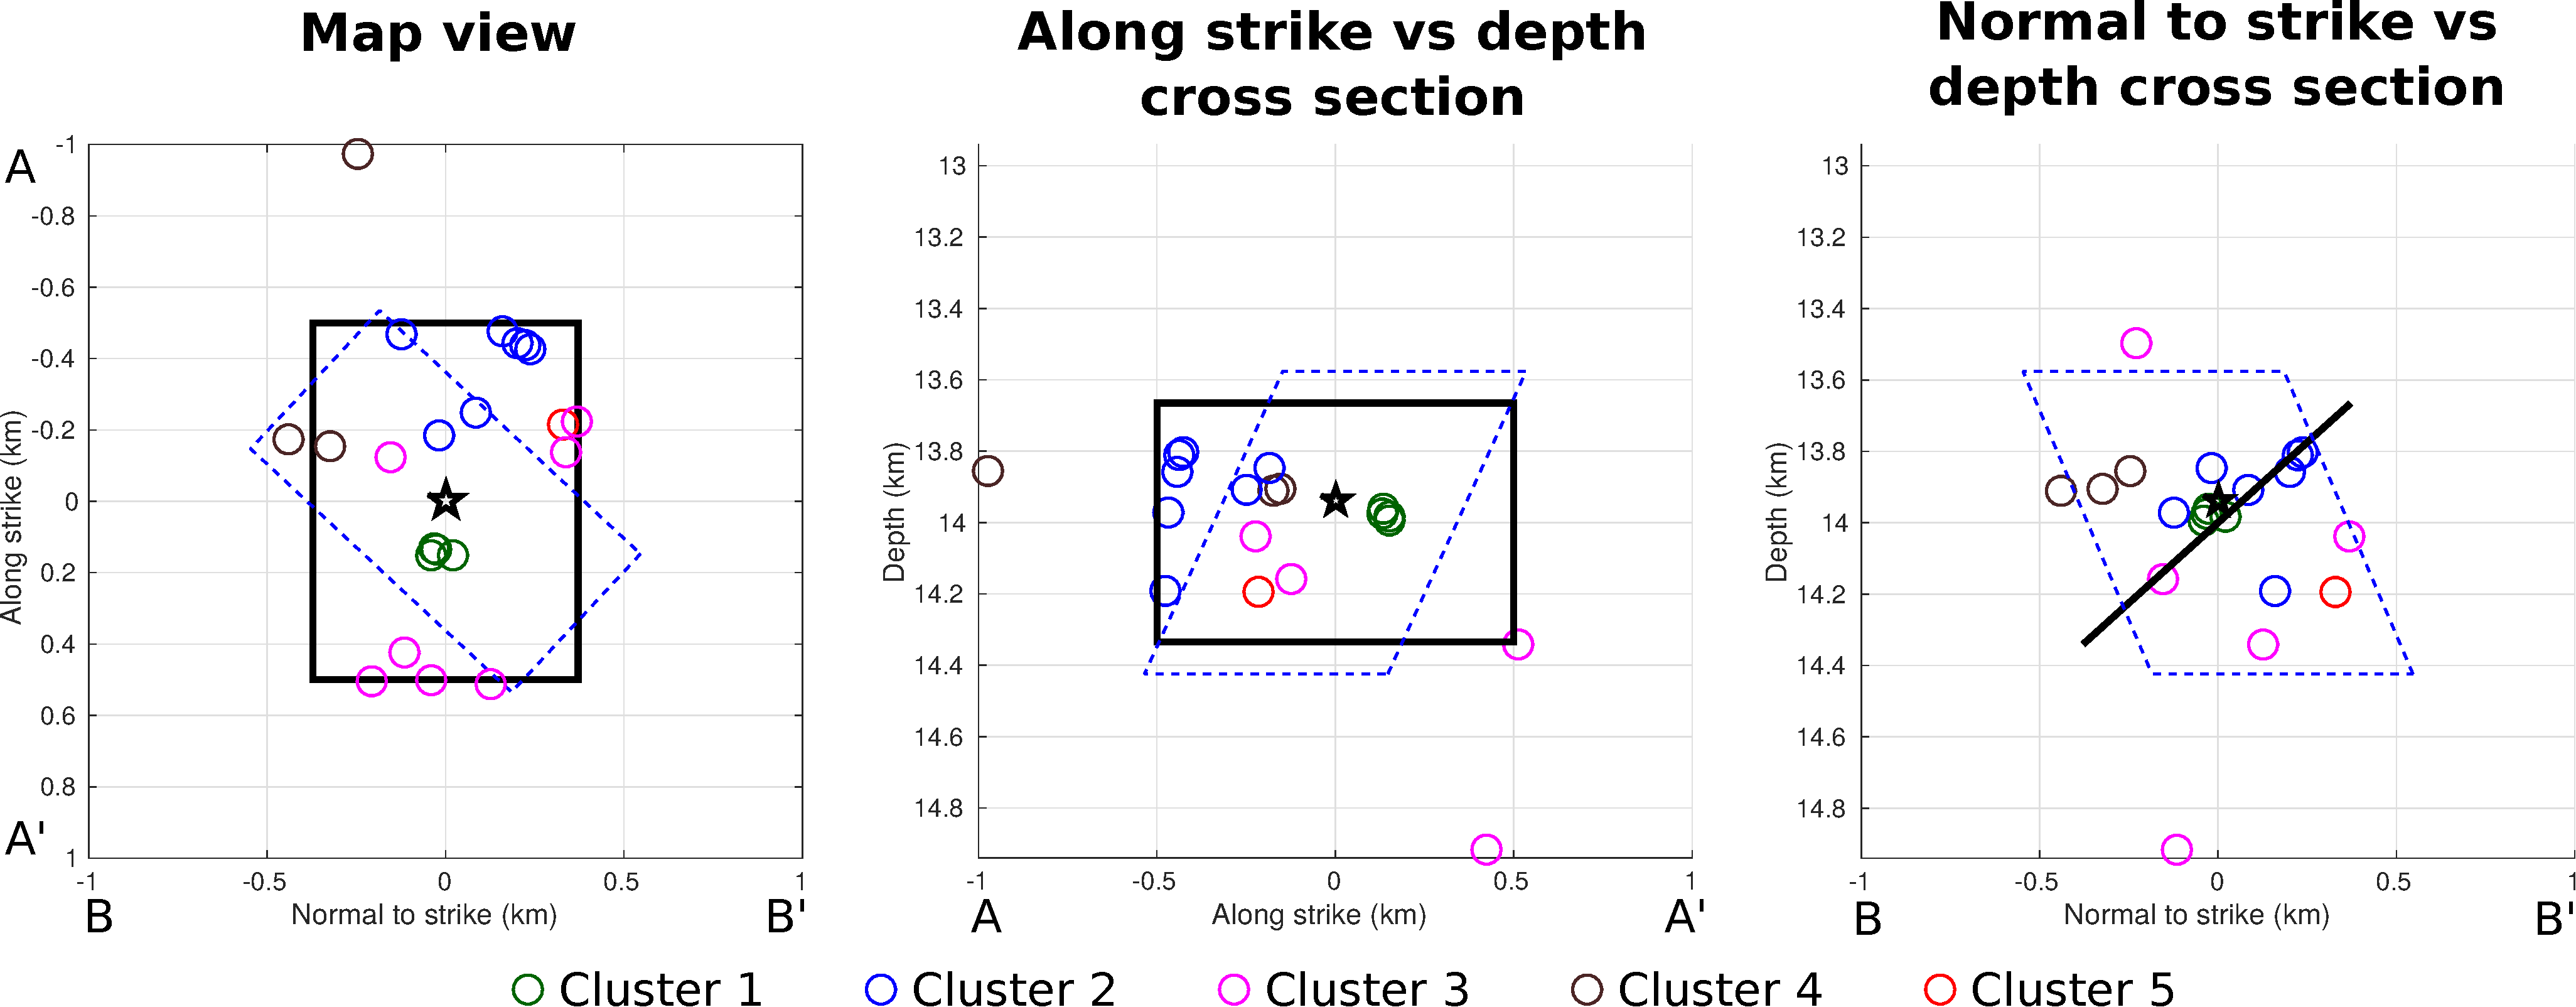
\includegraphics[width=1\linewidth]{images/S6_templates_per_cluster_map.pdf}
 \end{minipage} 
 
\end{frame}

\begin{frame}
 {Secuencia s\'ismica del sismo 2019 Mw4 Balsorano, Italia}

 \begin{minipage}{1\linewidth}
  \centering 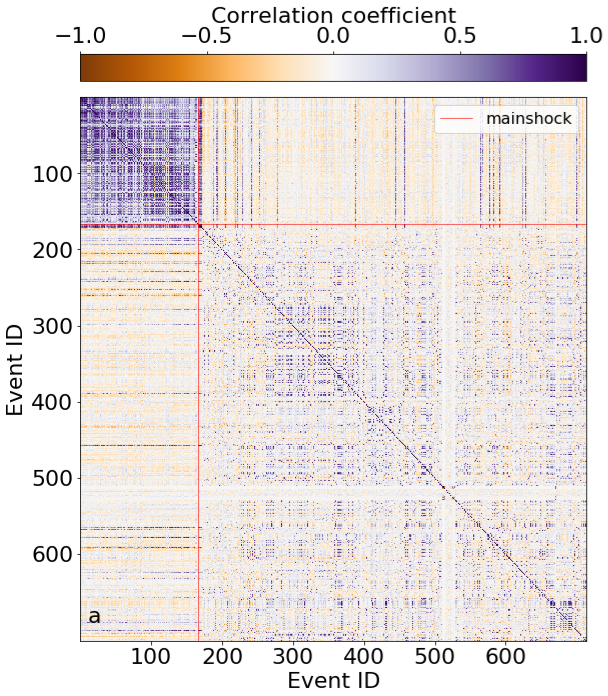
\includegraphics[width=0.65\linewidth]{images/matrix.png}
 \end{minipage} 
 
\end{frame}


\begin{frame}
 {Secuencia s\'ismica del sismo 2019 Mw4 Balsorano, Italia}

 \begin{minipage}{1\linewidth}
  \centering 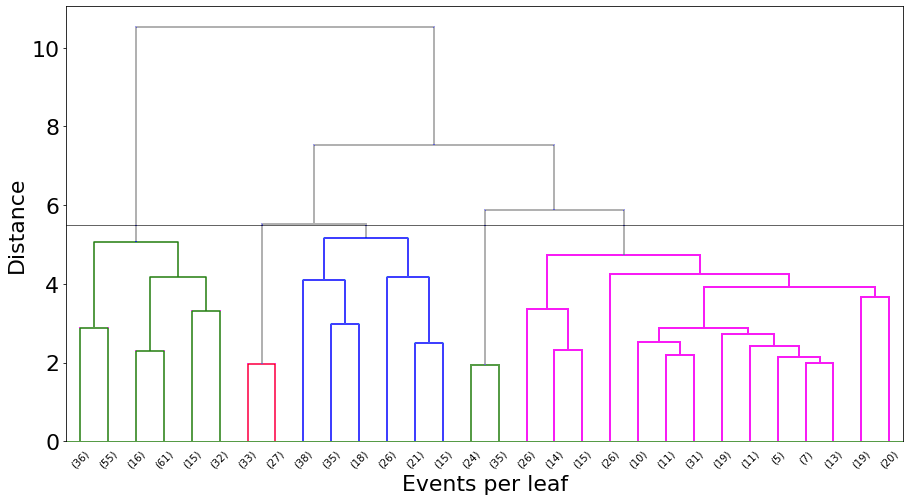
\includegraphics[width=1\linewidth]{images/dendrogram_balsorano.png}
 \end{minipage} 
 
\end{frame}


\begin{frame}
 {Secuencia s\'ismica del sismo 2019 Mw4 Balsorano, Italia}

 \begin{minipage}{1\linewidth}
  \centering 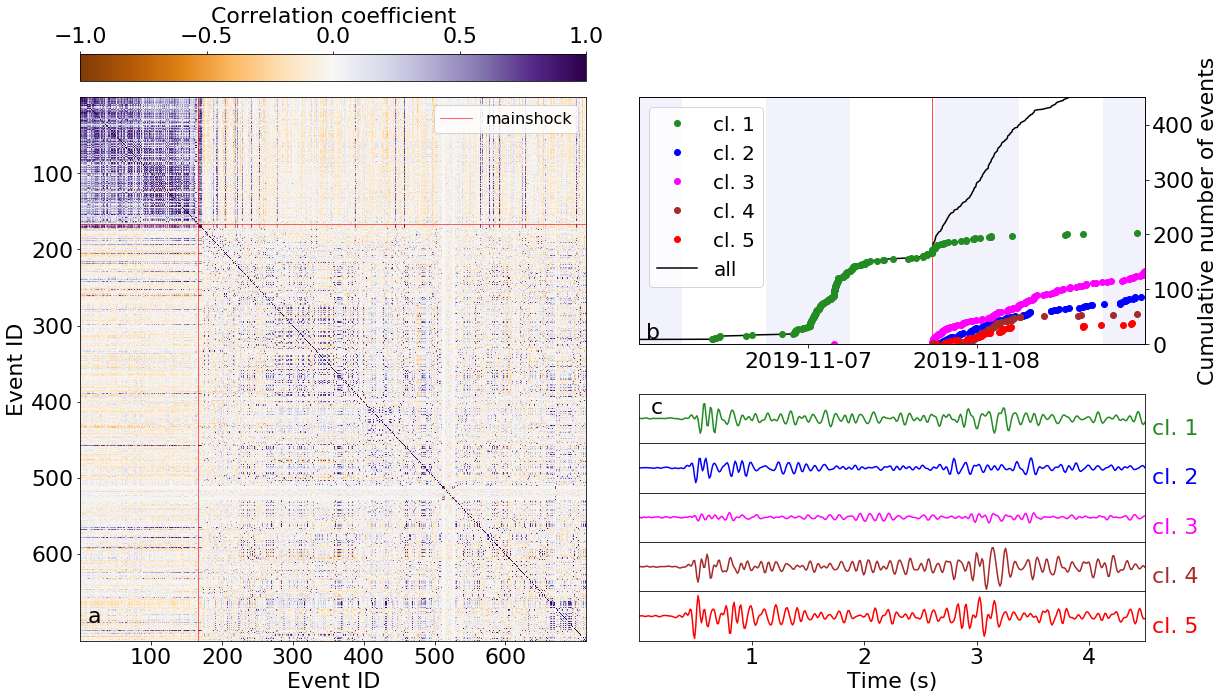
\includegraphics[width=1\linewidth]{images/wigg_cc_mat_cluster.png}
 \end{minipage} 
 
\end{frame}

\begin{frame}
 {Secuencia s\'ismica del sismo 2019 Mw4 Balsorano, Italia}

\vskip -0.2cm \begin{minipage}{0.48\linewidth}
   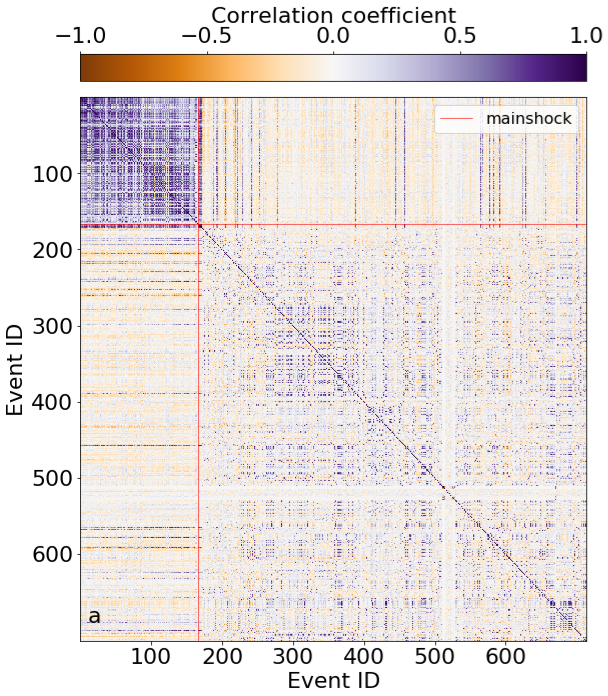
\includegraphics[width=0.95\linewidth]{images/matrix.png}
   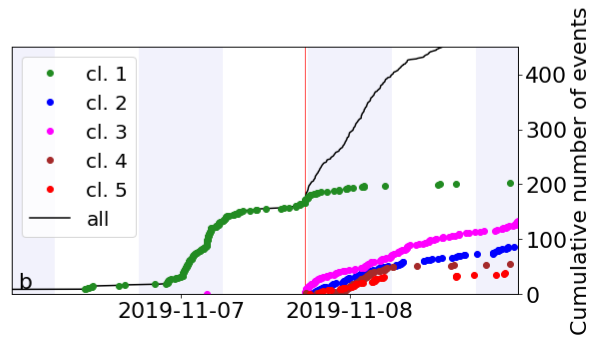
\includegraphics[width=0.95\linewidth]{images/cummulative.png}
 \end{minipage} 
 \begin{minipage}{0.5\linewidth}
   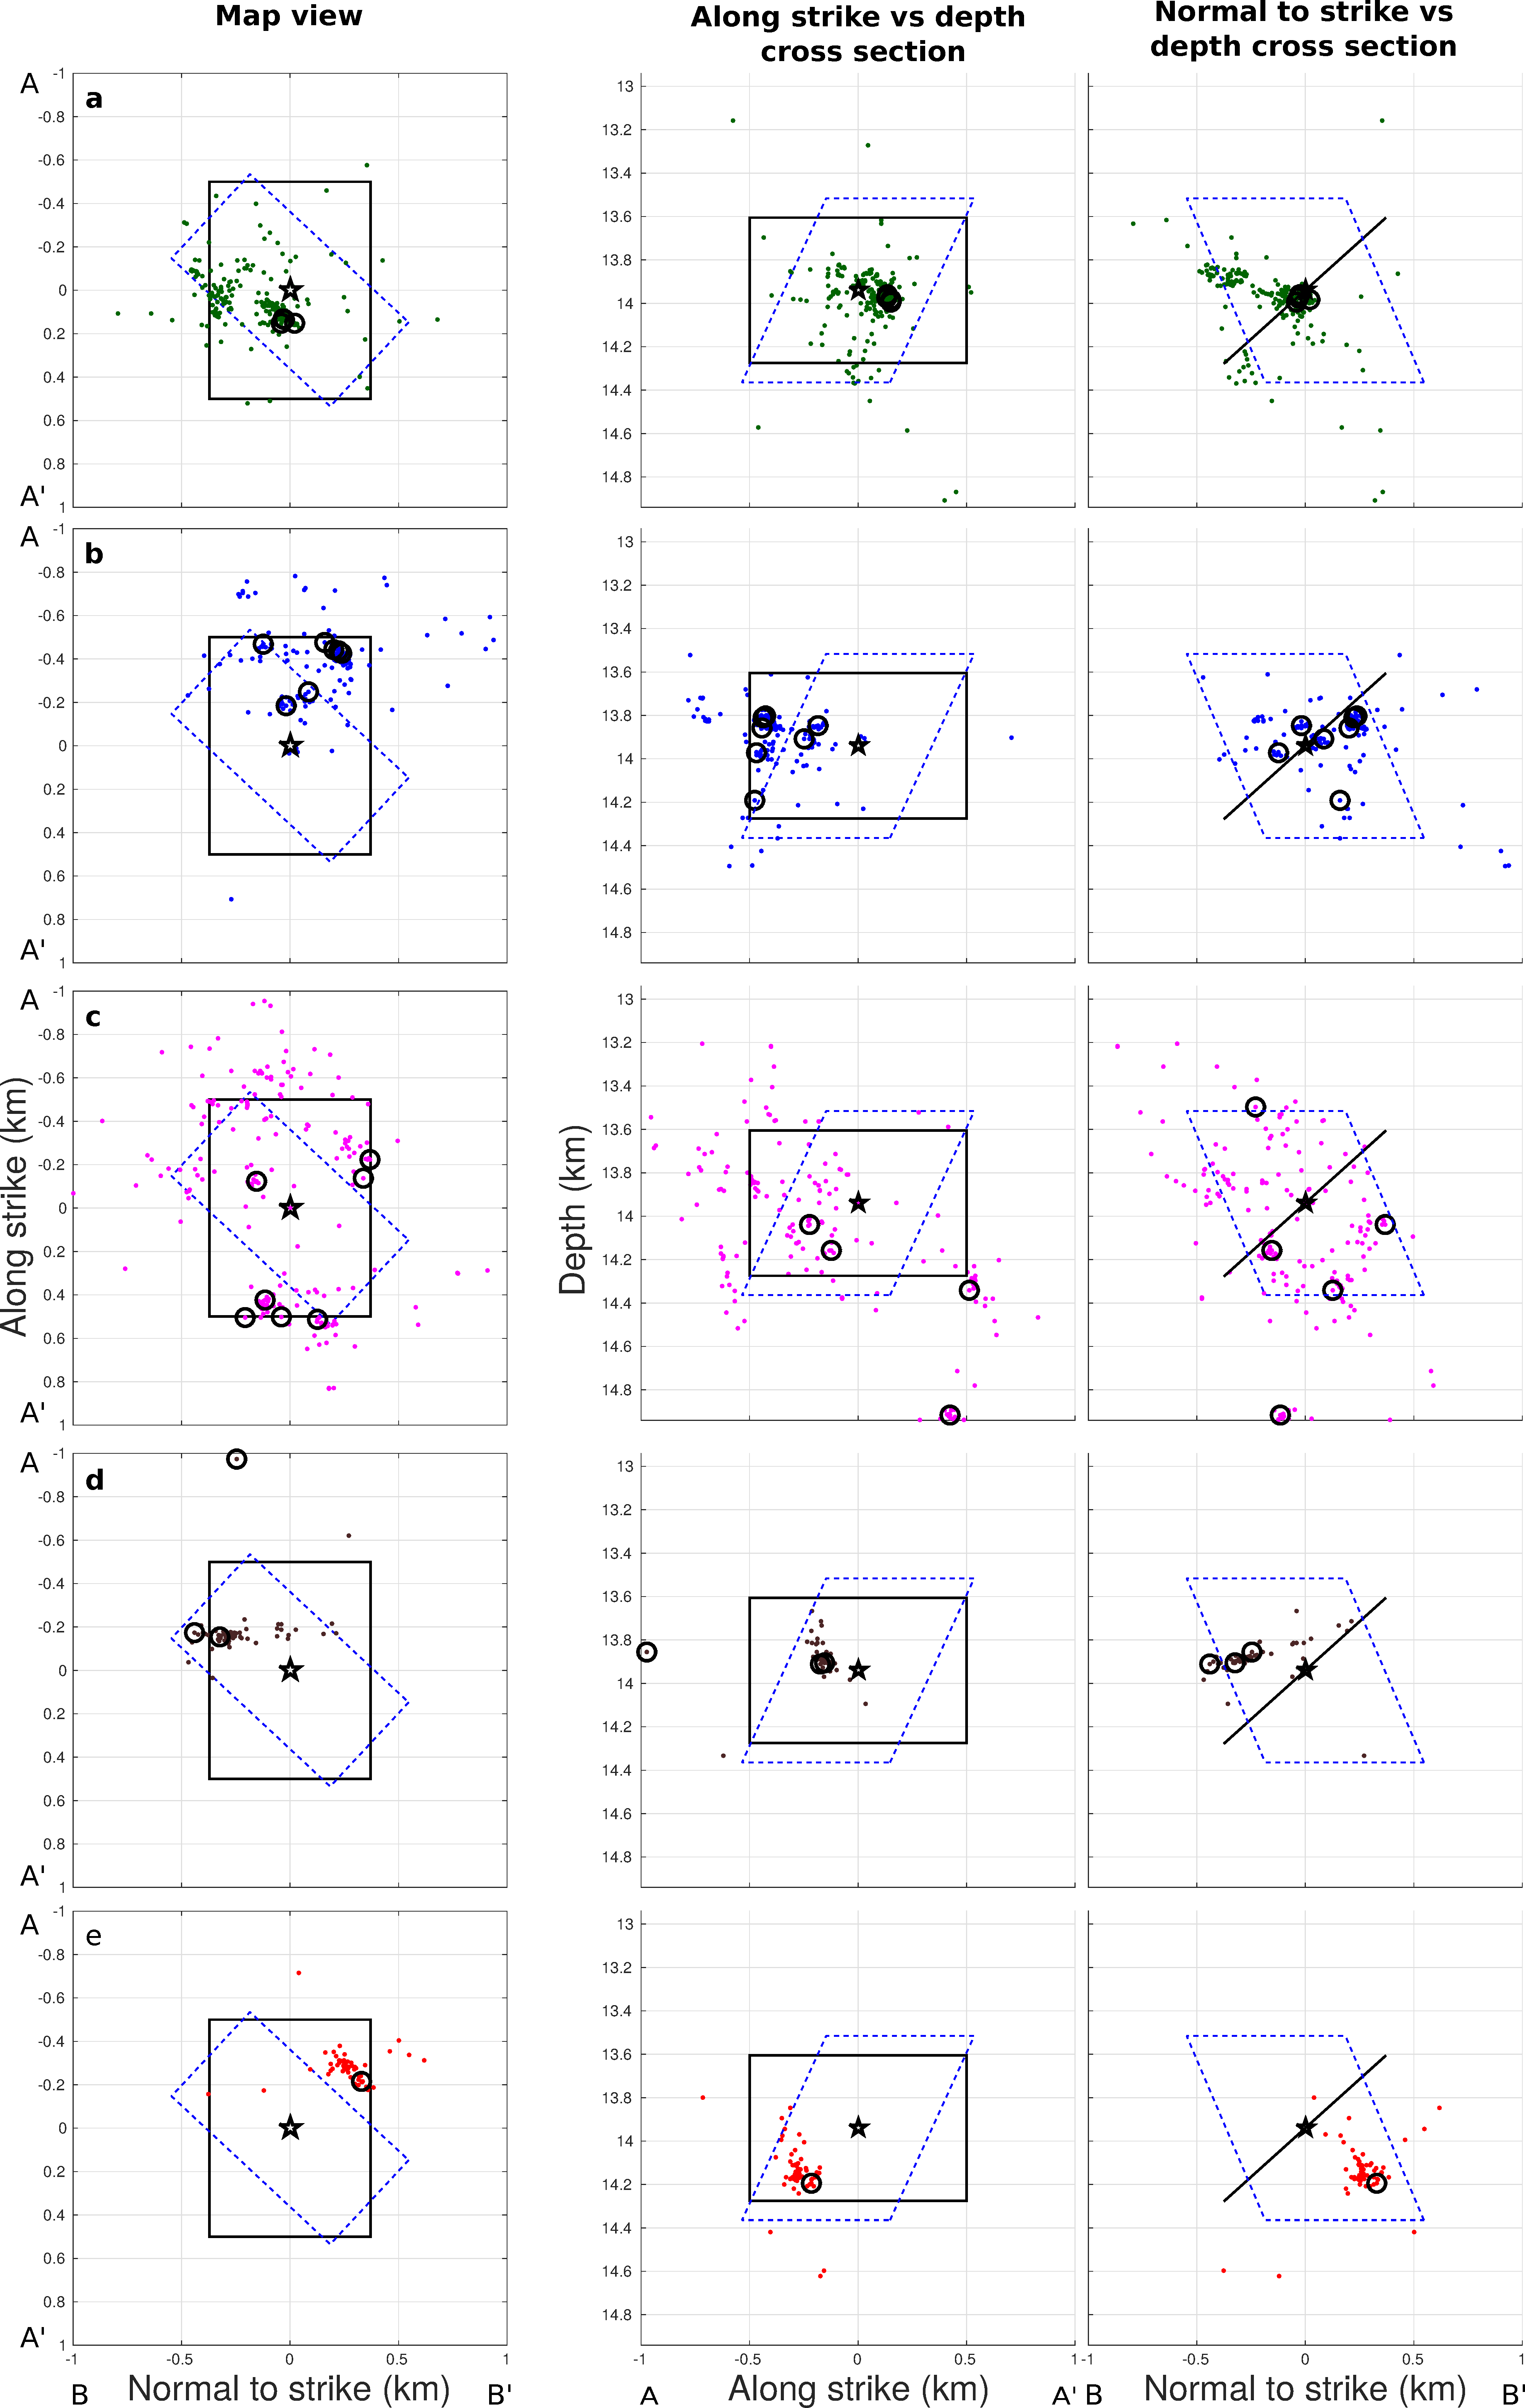
\includegraphics[width=0.95\linewidth]{images/map_clusters_templates.pdf}
 \end{minipage} 
 
\end{frame}




\section{Ejercicio}


\begin{frame}
 {Evento sísmico del 26 de Mayo del 2022, Mw7.2}
 
 \begin{minipage}{0.9\linewidth}
  \centering 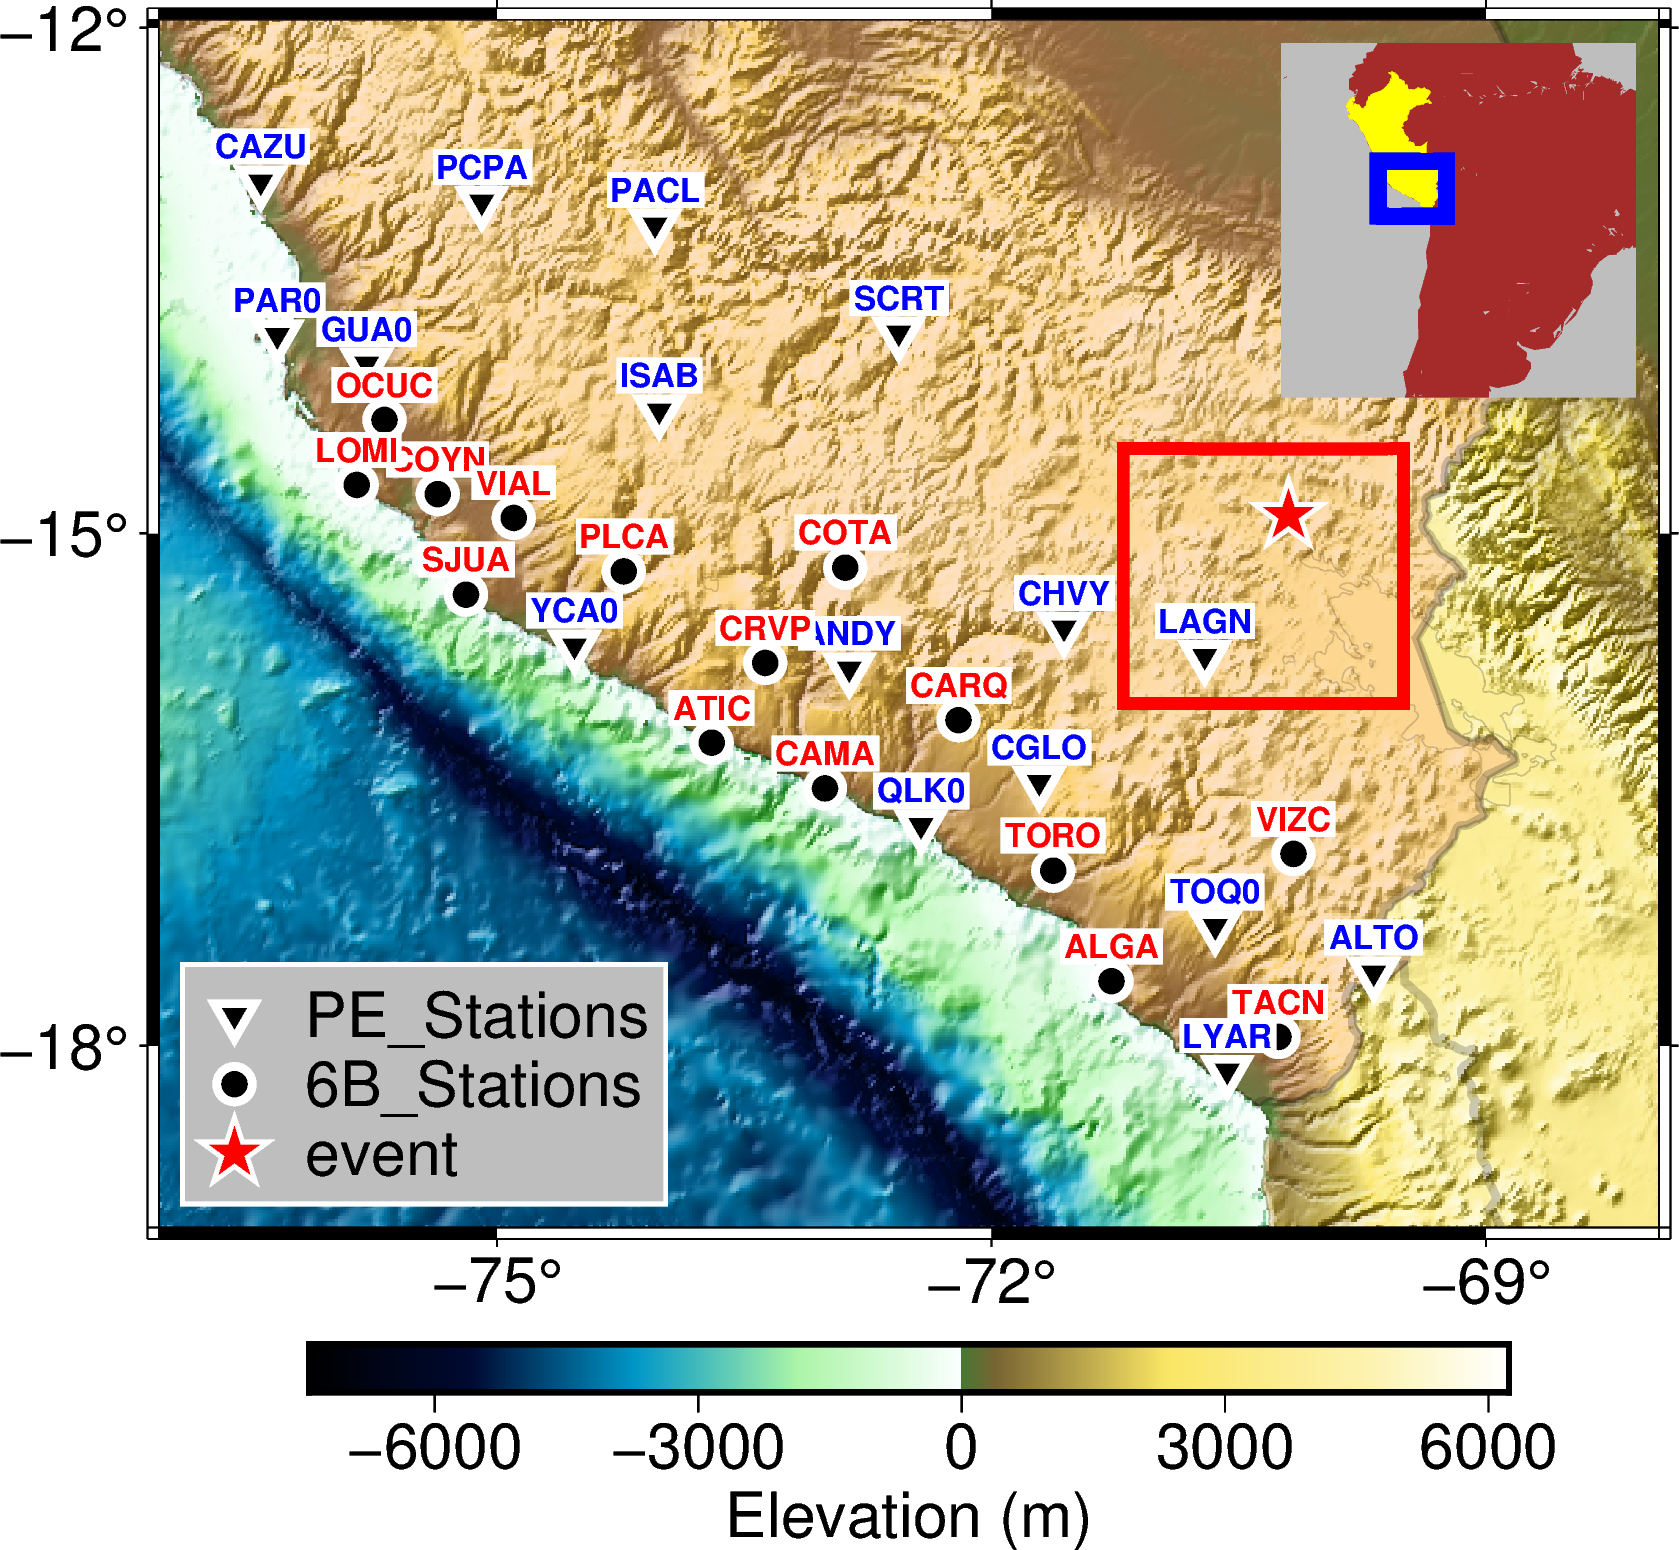
\includegraphics[width=0.9\linewidth]{images/map_peru}
 \end{minipage}
  
\end{frame}



\begin{frame}
 
 \begin{minipage}{1\linewidth}
  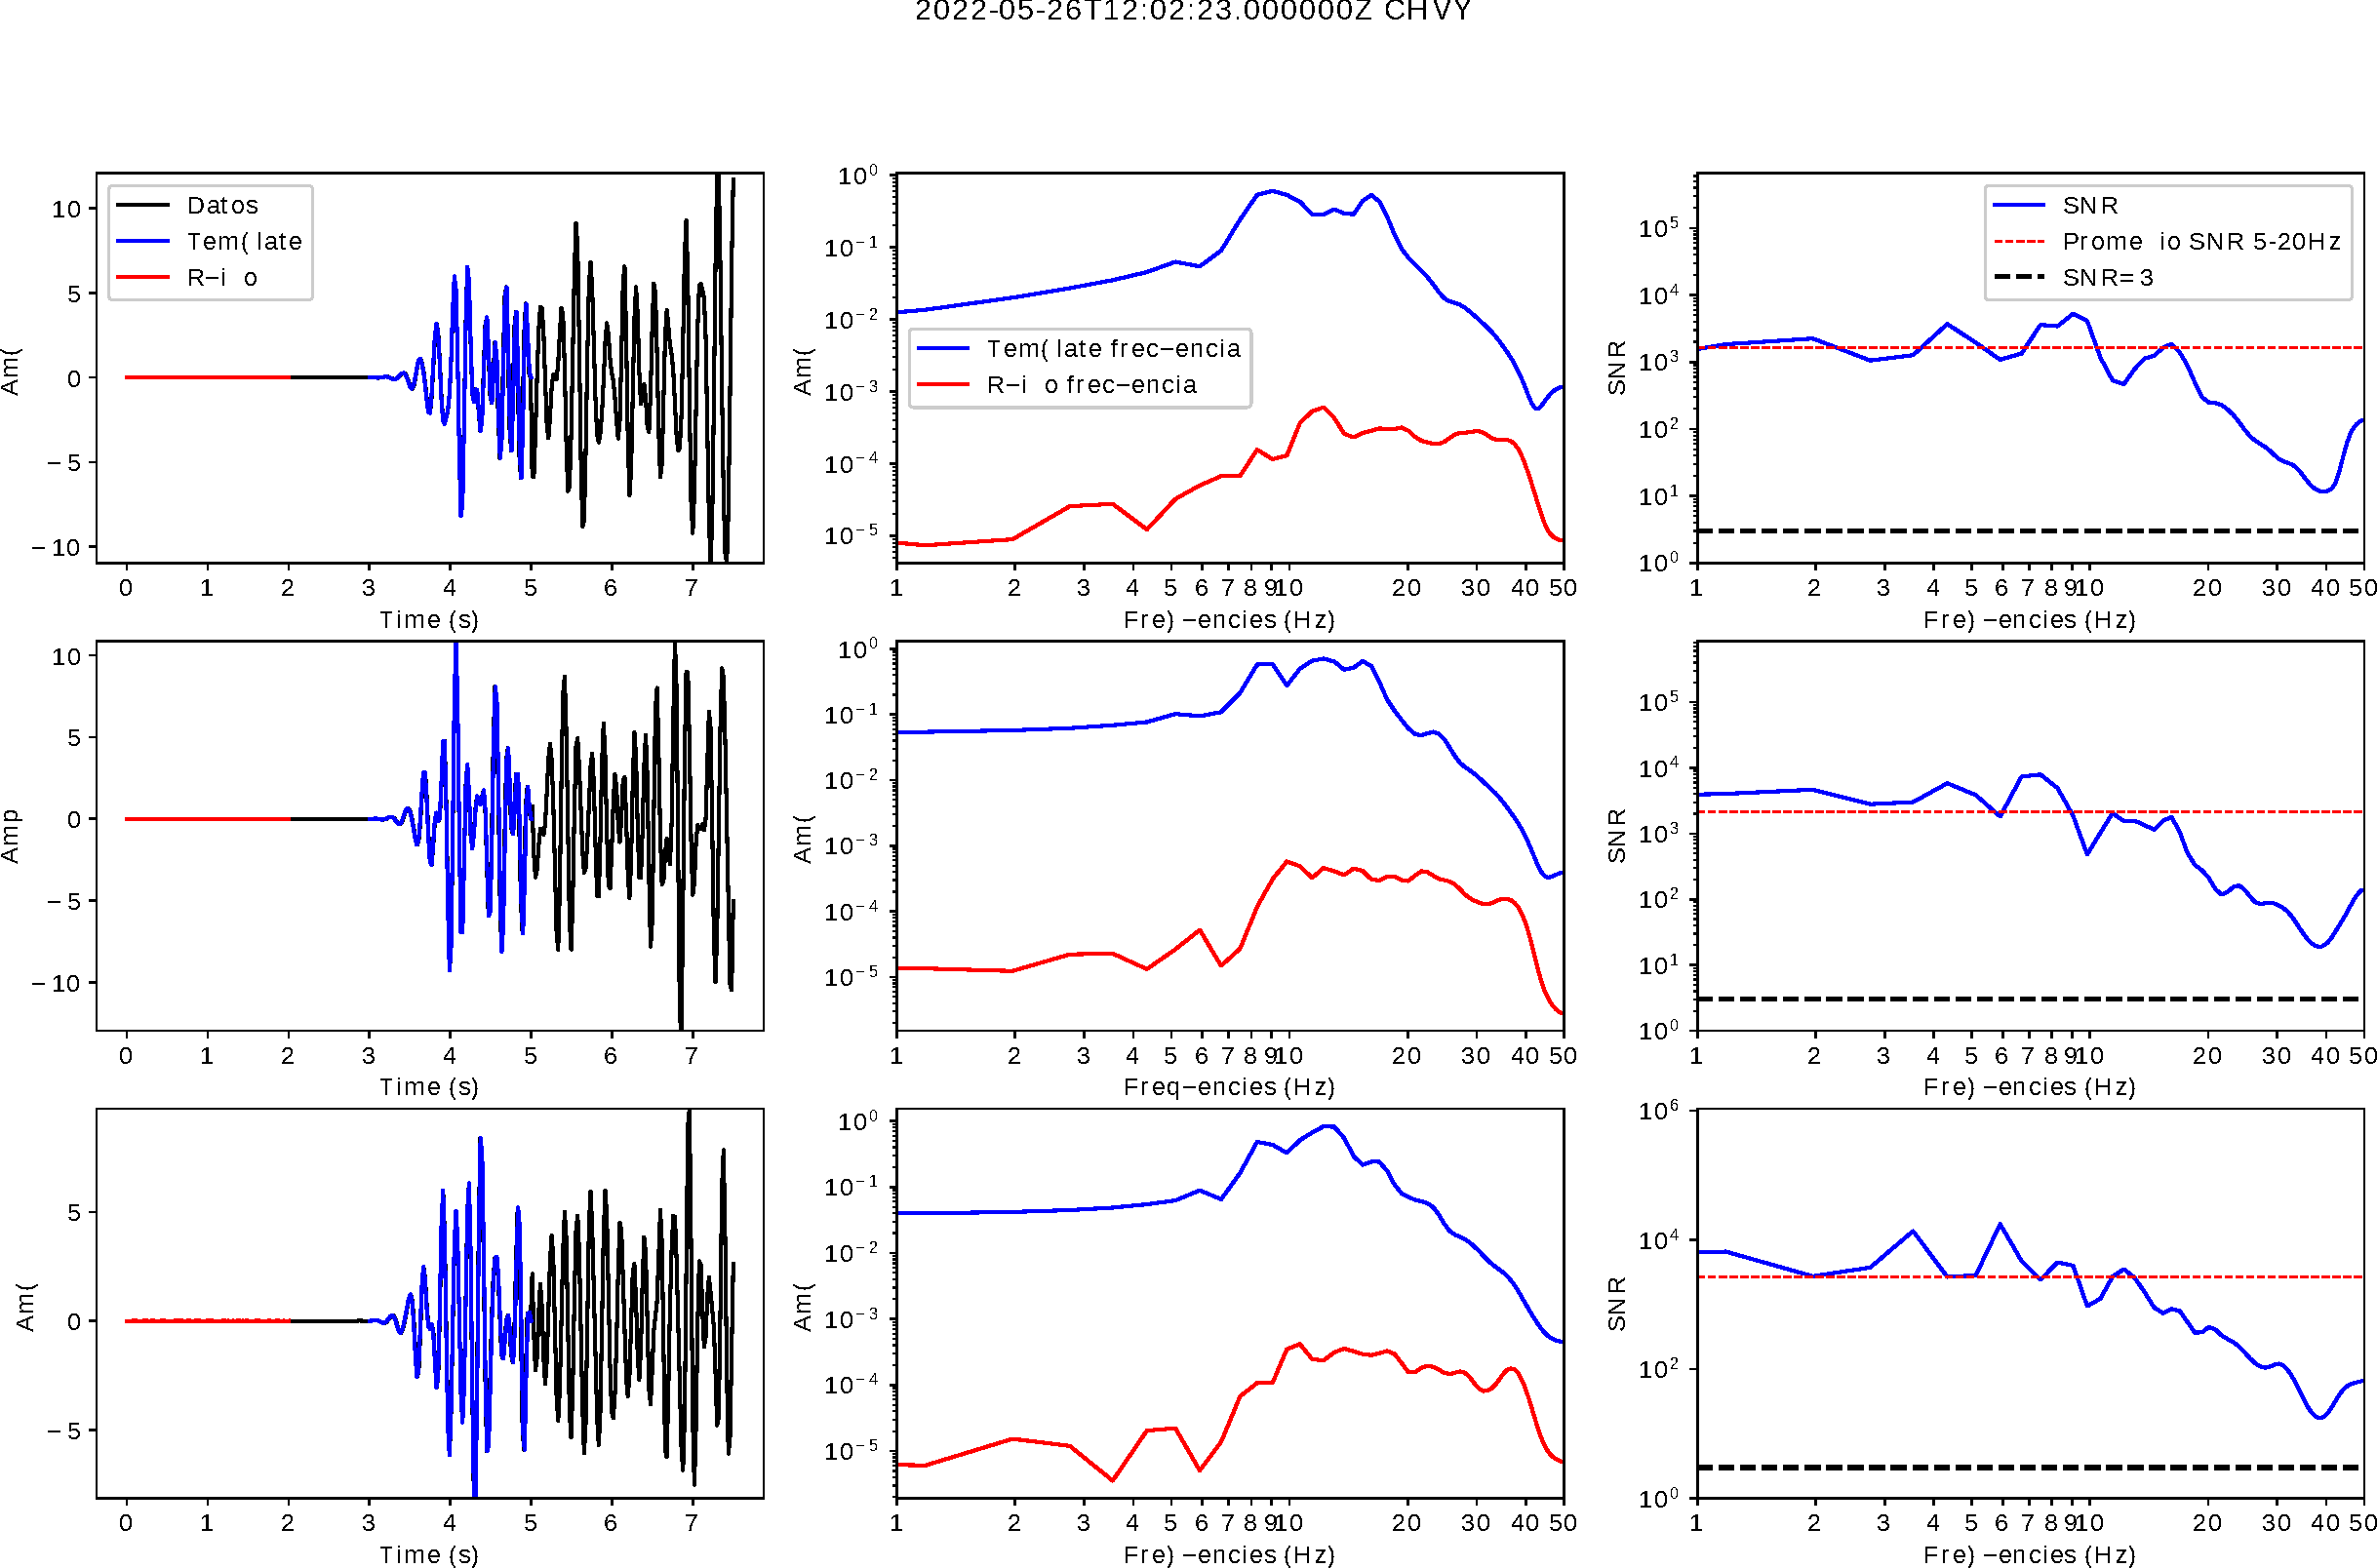
\includegraphics[width=1\linewidth]{images/snr_event_0_CHVY}
 \end{minipage}
 
\end{frame}




\end{document}

